\documentclass[10pt,conference,compsocconf]{./IEEEtran} 
%\documentclass[10pt,conference]{IEEEtran} 

\usepackage{setspace}
%\usepackage[firstpage]{draftwatermark}
\usepackage{epstopdf}
\usepackage{times}
\usepackage[table]{xcolor}
%\usepackage{url}
\usepackage[hidelinks]{hyperref}
%\usepackage{url}
\usepackage{comment}
%\usepackage[lofdepth,lotdepth]{subfig}
%\usepackage{floatrow}
\usepackage{graphicx}
\usepackage{fancyvrb}
\usepackage{listings}
\usepackage{rotating}
%\usepackage[usenames]{color}
\usepackage{setspace}
%\usepackage{tabularx,colortbl}
%\usepackage{subfigure}
\usepackage{subcaption}
\usepackage[noadjust]{cite}
\usepackage{multicol}
%\usepackage[usenames]{color}
%\usepackage{todonotes}
%\usepackage{enumitem}


\usepackage{amsmath}
\usepackage{booktabs, multicol, multirow}

% Used to balance last page
% \usepackage{flushend}

%\SetWatermarkText{PREPRINT}							
% correct bad hyphenation here
\hyphenation{op-tical net-works semi-conduc-tor}
%see http://tex.stackexchange.com/questions/62720/vertical-space-after-algorithm
\def\textfloatsep{6pt}
\def\intextsep{6pt}
\def\IEEEbibitemsep{0pt plus .5pt}
%%%%%%%%%%%%%%%%%%%%%%%%%%%%%%%%%%%%%%%%%%%%%%%%%%%%%%%%%%%%%%%%%%%%%%
%
% Program Float
%
\usepackage{float}

\floatstyle{ruled}
\newfloat{program}{thp}{lop}
\floatname{program}{Program}

%%%%%%%%%%%%%%%%%%%%%%%%%%%%%%%%%%%%%%%%%%%%%%%%%%%%%%%%%%%%%%%%%%%%%%
\begin{document}

\title{\huge{Automated Feedback-Based Vertical Elasticity for Heterogenous Soft Real-time Workloads}}

\author{
% Author Block
\IEEEauthorblockN{
\phantom{xxx}Yu-An Chen\IEEEauthorrefmark{1},
Andrew J. Rittenbach\IEEEauthorrefmark{2},
Geoffrey Phi C. Tran\IEEEauthorrefmark{2}\IEEEauthorrefmark{1},
John Paul Walters\IEEEauthorrefmark{2}, and
Stephen P. Crago\IEEEauthorrefmark{1}\IEEEauthorrefmark{2}\phantom{xxx}
}
\and
\IEEEauthorblockN{
}
\and
\IEEEauthorblockA{\IEEEauthorrefmark{1}Department of Electrical Engineering\\
University of Southern California,
Los Angeles, CA 90089\\
Email: \{chen116, geoffret\}@usc.edu}
\and
\IEEEauthorblockA{\IEEEauthorrefmark{2}Information Sciences Institute\\
University of Southern California,
Arlington, VA 22203\\
Email: \{aritten, gtran, jwalters, crago\}@isi.edu}

}
% \author{


% \IEEEauthorblockN{
% %Geoffrey Phi C. Tran\IEEEauthorrefmark{1}\IEEEauthorrefmark{2},
% \phantom{(Victor)}Yu-An Chen\IEEEauthorrefmark{2},
% %Dong-In Kang\IEEEauthorrefmark{1}, 
% % Mikyung Kang\IEEEauthorrefmark{1}, 
% John Paul Walters\IEEEauthorrefmark{1}, and
% Stephen P. Crago\IEEEauthorrefmark{1}\phantom{(Victor)}
% }
% % \and
% % \IEEEauthorblockN{
% % \phantom{(Victor)}
% % }
% % \IEEEauthorblockN{
% % }
% \and
% \IEEEauthorblockA{\IEEEauthorrefmark{1}Information Sciences Institute\\
% University of Southern California,
% Arlington, VA 22203\\
% Email: \{jwalters, crago\}@isi.edu}
% % gtran dkang, mkkang, jwalters, crago
% \and
% \IEEEauthorblockA{\IEEEauthorrefmark{2}Department of Electrical Engineering\\
% University of Southern California,
% Los Angeles, CA 90089\\
% Email: chen116@usc.edu}
% % geoffret chen116

% }

\maketitle


\begin{abstract}
Cloud computing provides a pool of highly available resources for applications to offload their tasks to, but new applications such as coordinated lane change assistance used in connected car system have strict timing requirements that cannot be met by offloading tasks only to the cloud. Fog computing reduces latency by bringing the computation from remote datacenter to local fog servers, which are connected in close proximity with the clients.  Although fog computing lowers the latency for transferring data, load balancing among fog servers still needs to be addressed for better timing performance. The challenges include large number of tasks, mobility of the clients, and the heterogeneity of the fog servers. In this paper, using connected car systems as a motivating application, we first show that we can utilize mobility patterns of vehicles to perform periodic load balancing in fog servers. We then present a task model that solves the scheduling problem at the server level instead of device level. And finally we formulate a load balancing optimization problem for minimizing deadline misses and total runtime for connected car system in fog computing. We show that it outperforms some common heuristics such as weighted round robin, active monitoring, and throttled load balancer.

\iffalse In fog computing, servers and the clients are connected in close proximity. Computation is brought from the remote datacenter to local servers, thus data can be processed and response faster. Applications cloud provides a pool of highly available resources for applications to offload their tasks to, but new applications such as coordinated lane change assistance for self-driving car has strict timing requirements that cannot be met by only running it in the cloud. Although fog computing lowers the latency for transferring data, load balancing and task distribution within local servers still need to be addressed for better timing performance. The challenges of minimizing deadline misses and runtime in fog computing come with the mobility of the clients, high number of tasks, and the heterogeneity of the local fog servers. In this paper, using lane change assistance for self-driving car as example application, we first show that we can use mobility of cars to perform periodic online scheduling in local servers. Secondly, we present a task scheduling model that can reduce the problem size. And finally we propose a task distribution optimization formulation that outperform commonly used load balancing algorithm such as weighted round robin, active monitoring, and throttled load balancer.
\fi

\iffalse Applications offload tasks to the cloud for its highly available resources and fast processing speed. But new applications such as coordinated lane change assistance for self-driving car has stricter timing requirements that cannot be met by offloading tasks to the cloud. In fog computing, fog servers and the clients are connected in close proximity. Computation is brought from the remote datacenter to local servers, thus data can be processed and response faster. The challenges of minimizing deadline misses and runtime in fog computing come with the mobility of the clients, high number of tasks, and the heterogeneity of the local fog servers. In this paper, using lane change assistance for self-driving car as example application, we first show that mobility of cars can be predicted with high accuracy ~95\% with a simple linear prediction mechanism.  Secondly, we present a task scheduling model that can reduce the problem size. And finally we propose a task distribution optimization formulation that outperform commonly used load balancing algorithm such as weighted round robin, active monitoring, and throttled load balancer.
\fi


\end{abstract}

\begin{IEEEkeywords}
fog computing; load balancing; real-time; task distribution; deadline misses; connected car; mobility prediction
\end{IEEEkeywords}

\section{Introduction}



sdf
\iffalse
\begin{enumerate}

%\item We propose a task model that provides a platform to develop load balancing algorithm that does not require the knowledge of how individual task is scheduled by moving the scheduling problem from device level to server level.
\item We propose a task model that provides a platform to develop load balancing algorithm that does not require the knowledge of how an individual task is scheduled by moving the scheduling problem from device level to server level. It is impractical to obtain the scheduling information about each task because the traffic of the network make the arriving order of tasks a stochastic process and the problem size increase more rapidly.
\item We propose an optimization problem formulation for load balancing that minimizes deadline misses and total runtime for connected car system in fog computing.
\end{enumerate}

The rest of the paper is organized as follows: we review existing works in load balancing for mobile clients in fog computing in Section \ref{s1}. In Section \ref{s2}, we present a simple linear mobility prediction algorithm with high accuracy to show that online task scheduling is beneficial in fog computing. We present our task model and optimization problem formulation in Section \ref{s3}. In Section \ref{s4}, we analyze the performance of the optimization problem formulation. Conclusions and future work are discussed in Section \ref{s5}.


\fi


\section{Related Work}


DART-C,POET, other POET, 
Adaptive Management of Virtualized Resources in Cloud Computing Using Feedback Control

Priority Based Dynamic Resource Allocation in Cloud Computing with Modified Waiting Queue

Adaptive Control of Virtualized Resources in Utility Computing Environments 

Active Resource Allocation Management in Virtual Cloud Instances

Dynamic virtual machine allocation policy in cloud computing complying with service level agreement using CloudSim

Vertical and horizontal elasticity for dynamic virtual machine reconfiguration

Automatic memory-based vertical elasticity and oversubscription on cloud platforms







\iffalse



\label{s1}
%The research challenges for load balancing comes with the heterogeneous and decentralized nature of fog computing. There are many existing works that aim to solve task distribution with different emphasis, application examples and solutions. 



% Oueis et al. \cite{thef} solve the resource allocation problem for grid computing in a building. In grid computing, each node is connected wirelessly so the optimization formulation focus on both computational and radio resources allocation to minimize power consumption per node while satisfying all the latency constraints imposed by each node. The difference between our work and their work is that they put emphasis on radio resource allocation, impose only hard deadline constraint.




In the work of Oueis et al. \cite{fogba}, they construct two optimization problems that minimize total transmitting power and total computation time respectively. In their work, tasks can be partitioned to servers and constrainted to hard deadlines, whereas tasks are indivisible and have soft deadlines in our work. Zeng et al. \cite{jopt} formulates a linear program that aims to minimize the average task completion time, but we also focus on avoiding missing deadlines for each task in our formulation.


Hong et al. \cite{smallfogcar} propose a programming model that uses the workload to dynamically scale the fog system in order to provide enough resources. Their example applications include vehicle-to-vehicle video streaming and traffic monitoring. The difference between our work and theirs is our work consider deadline constraint and placements of individual task to the fog servers while theirs does not.


Takayuki et al. \cite{serviceo} use routing for smart cars as the application that is being offloaded to the fog servers. Their load balancing optimization formulation focuses on minimizing aggregated task finishing time under an energy constraint. The difference between our work and theirs is that they do not impose capacity or resource constraint on the servers while we do. %They also do not consider the fact that a node assigned with multiple tasks will have a non-uniform response time to each task. 


Hong et al. \cite{oppos} use the car's mobility patterns to predict its future location and then forward the tasks to the fog server that is associated with predicted location so the processing can start without any delay when the car arrives. The tasks include gathering and processing the data from local sensors. Their work has similar approach to our work in that they utilize mobility but their system focuses on only single client and does not impose capacity/resource constraints on the servers while we work with a multi-clients system that have various contraints on the servers. 

% Deng et al. \cite{optimalw} suggest many different types of applications that can utilize fog computing for local processing such as geographically distributed applications such as pipeline monitoring networks and large-scale distributed control systems such as smart energy distribution, smart traffic lights and connected vehicles. They propose a load balancing optimization for optimal task placement in the fog nodes and remote cloud to minimize energy usage. The difference between our work and their work is that their formulation focuses more on minimizing power and has all tasks finish before deadline as constraints. 


In the work of Wang et al. \cite{onlinep}, they use face recognition running on mobile devices as the motivating application. Their approach is to treat tasks coming from mobile devices as a tree graph, and then solve for the optimal matching of those task nodes to the physical nodes. Their solution is to assign weighted costs for placing an application node to a physical fog node then find the optimal mapping that minimizes total cost. The difference between our work and theirs is our work accounts for timing constraints and multi-user models while theirs does not.


Li et al. \cite{energya} solve the problem of how to partition tasks for local servers and remote cloud to process and then allocate resource based on the partitioning. Video streaming on mobile devices is the example application. They propose an optimization formulation to minimize finishing time, cost of processing, and bandwidth usage. One major difference between our work and their work is that their formulation does not allow any deadline misses while our work tries to minimize deadline misses.




\fi









\section{Mobility Pattern Prediction}
\label{s2}

\subsection{Connected Car System Model in Fog Computing}


Many works have been done in mobility prediction in vehicles using methods such as Markov Chain\cite{sf} or probability distributions\cite{rome}. In this section we will show that even a simple linear model can give high prediction accuracy such that task allocations based on mobility prediction is practical.

First we present a model for a connected car system in fog computing. An example model is illustrated in Figure \ref{carrep}. In Figure \ref{carrep}, A, B, and C represent three different fog servers and each car is counted as a client. Each fog server manages the cars that are within its wireless range. We assume the wireless communication protocol used between cars and servers is 802.11p, Wireless Access in Vehicular Environments (WAVE)\cite{wave}, which has communication range of at least 500 meters or above\cite{waver}. We also use a hexagon to indicate the wireless coverage area of a fog server instead of omnidirectional coverage because hexagonal cell shape approximation is more suitable for implementing wireless network system\cite{hex}. 

\begin{figure}[h!]
\centering
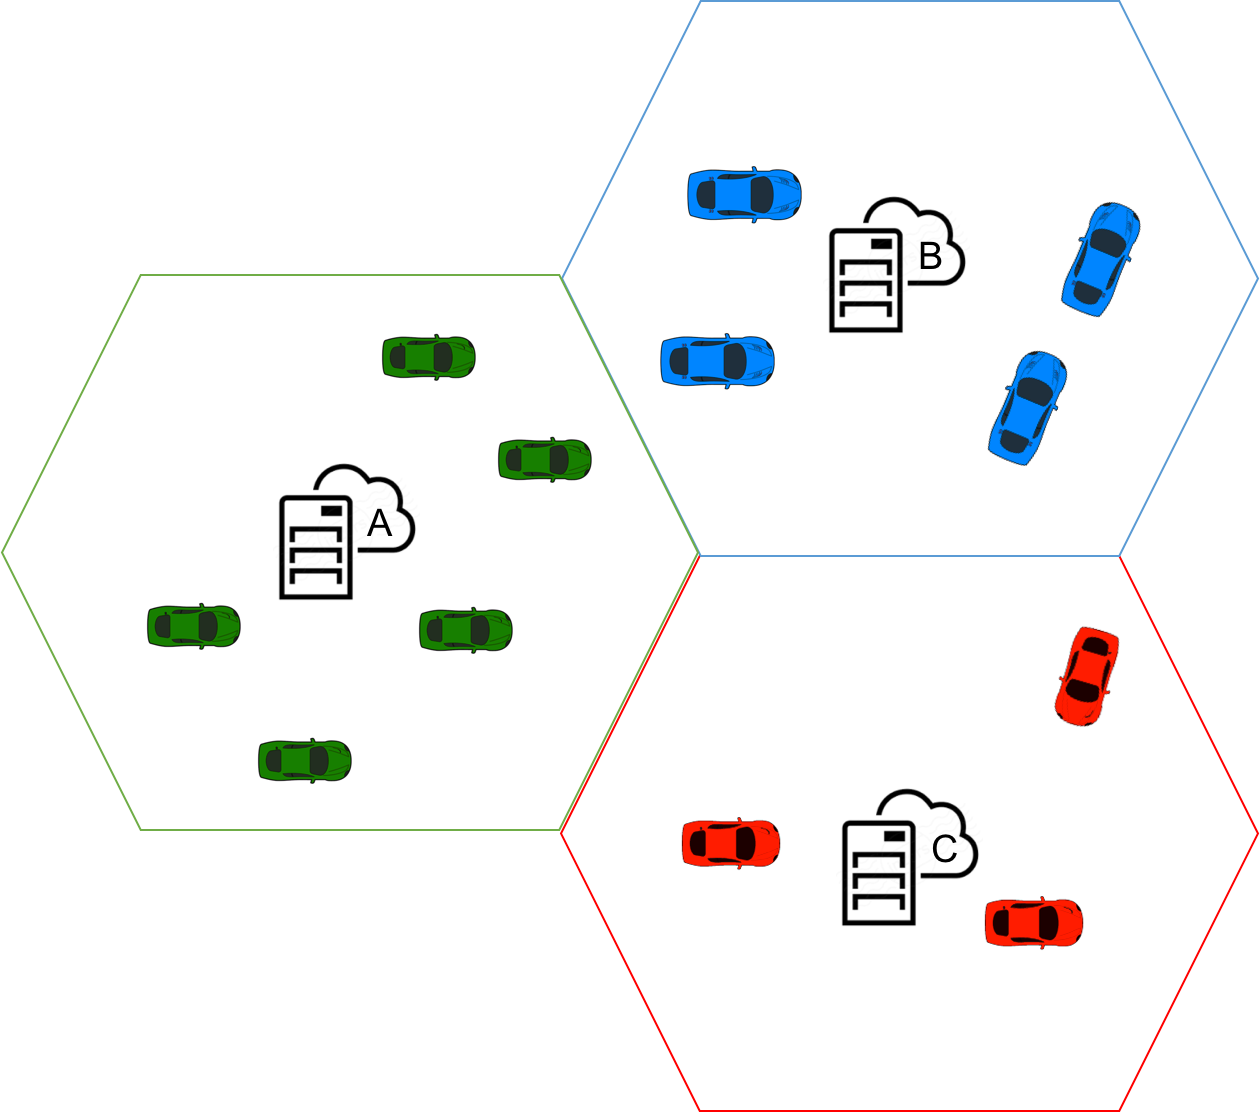
\includegraphics[width=0.75\linewidth]{images/car_rep}
\caption{Example Fog Computing Model}
\label{carrep}
\end{figure}



\subsection{Linear Mobility Pattern Prediction}
\label{background:model}
We propose a linear mobility prediction algorithm that uses just previous location and current location of a car to predict its future location. Assuming each car updates its location every $\theta$ seconds, when a car updates its location at time $t$, the corresponding fog server uses the car's previous location and timestamp to calculate the car's current speed and direction. The predicted location for the car will be the position of the car at time $t+\theta$ with current speed and direction. If the predicted location is outside of the current fog server's wireless range, then the algorithm will determine which server the car will travel to by finding the neighboring server that is the closest to the car’s predicted location. Figure \ref{carmodelrep} shows a graphical illustration of the prediction algorithm. 

\begin{figure}[ht!]
\centering
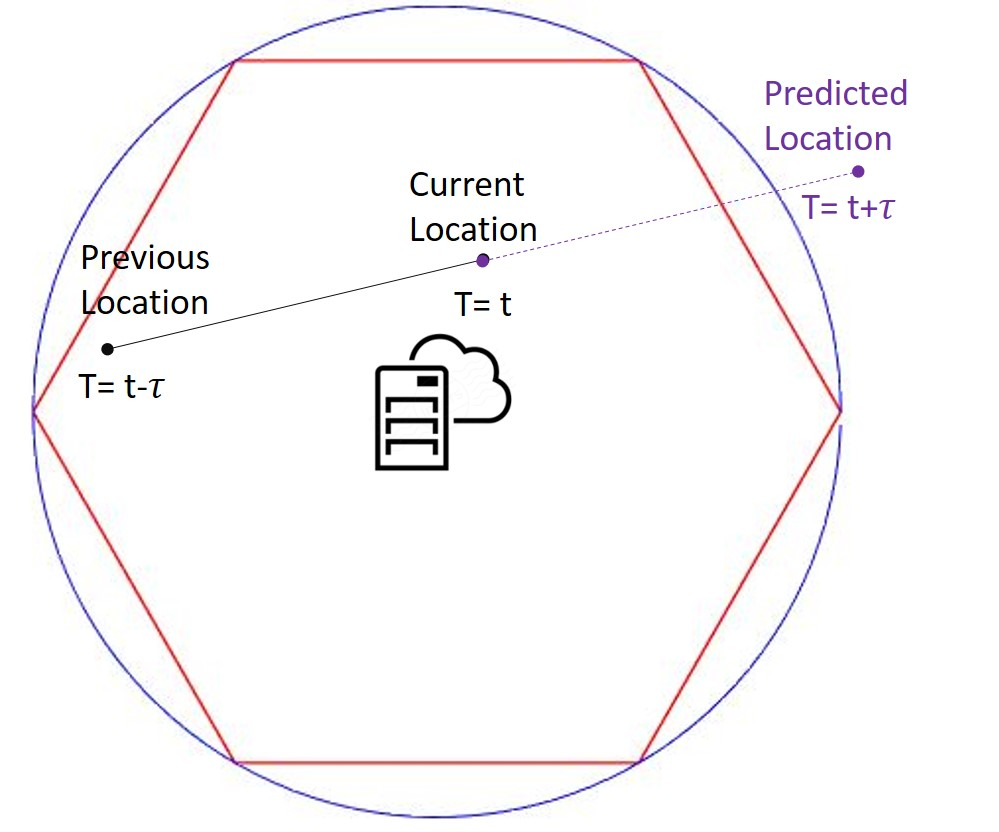
\includegraphics[width=0.5\linewidth]{images/car_model_rep}
\caption{Mobility Prediction Algorithm}
\label{carmodelrep}
\end{figure}


We test our linear prediction algorithm with real GPS data of taxis gathered in Rome, Italy\cite{romet}. The update period for the dataset is about 7 seconds. We divide up the region into a system with 7 fog nodes each with radius of 500 meters, as shown in Figure \ref{car7}. We use our linear prediction algorithm to keep track of the taxis' mobility pattern, and notify the system when the algorithm anticipates a taxi is leaving or entering the wireless coverage of the center fog node by predicting which of the 6 regions the taxi is heading toward or coming from. The result is shown in Figure \ref{RomeRes}, where the blue lines indicate correct predictions and red lines indicate incorrect predictions. We are able to obtain a 94.89\% accuracy as shown in Table \ref{cartable}. In the next section, we will present a task model based on the model presented in this section, and then develop an optimization problem formulation for load balancing that minimizes deadline misses and total runtime.


\begin{figure}[ht!]
\centering
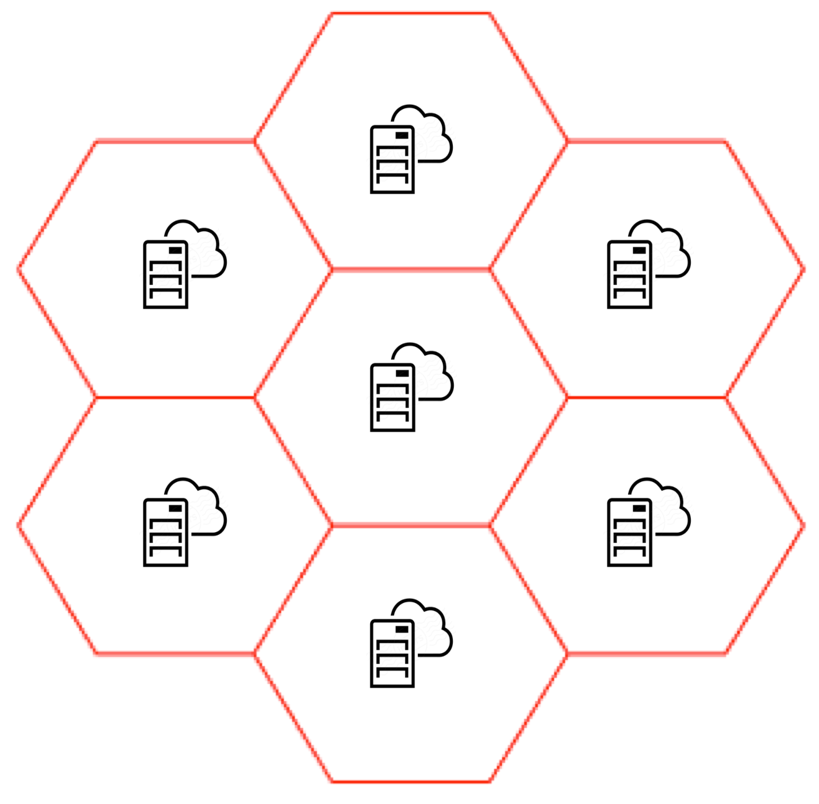
\includegraphics[width=0.5\linewidth]{images/car_7}
\caption{A Fog System with 7 Fog Nodes}
\label{car7}
\end{figure}


\begin{figure}[ht!]
\centering
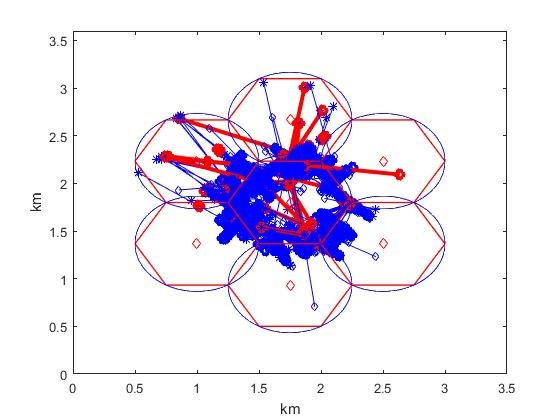
\includegraphics[width=1\linewidth]{images/car_res}
\caption{Linear Prediction Graphical Result}
\label{RomeRes}
\end{figure}


\begin{table}[h]
%\small
\caption{Linear Prediction Numerical Result}
\centering
\begin{tabular}{|m{4cm}|m{2cm}|}
	\hline
	Correct Preditction Count & 2505 \\ 
	\hline
	Total Prediction Count & 2640 \\ 
	\hline
	Accuracy & 94.89\% \\ \hline
\end{tabular}
\label{cartable}
\end{table}




















\section{Load Balancing in Fog computing}
\label{s3}

\subsection{Fog Computing Task Model}
\label{Fog Computing Task Model}

% We showed that it is possible to obtain fairly high accuracy with simple linear prediction model. 


In section \ref{s2}, we show that vehicles' mobility pattern can be predicted with high accuracy. For a application such as lane change assistance in connected car, we want to have the data ready for a car when it connects with a new fog server. With the ability to predict which server a car is traveling to, we can perform load balancing and process the tasks before the cars arrive at their predicted locations. 

The task model for connected car system in fog computing is composed of cars, local fog servers and a remote cloud server. The local servers are inter-connected and also connected to the cloud server. A simple system can be illustrated using Figure \ref{opt_rep}. In Figure \ref{opt_rep}, there is one cloud server and three local fog servers, A, B and C. Each fog server is connected to the cars that sit in its wireless range, indicated by hexagons with different colors. We treat the workload from each car as one task. Those tasks are passed through the nearest servers, which can either keep the tasks and do the processing or distribute them to other servers that have extra capacities. So in Figure \ref{opt_rep}, 5 tasks are initially passed to server A, 3 tasks are initially passed to server B and, 4 tasks are initially passed to server C, and the cloud server does not get any initial task.


The general graphical representation of the task model is shown in Figure \ref{opt_gen}. The local servers are interconnected, so they can distribute their tasks among themselves or the remote cloud. In other words, all servers can both accept tasks from other servers and offload tasks to other servers. Each server can have different resources and constraints. Table \ref{fogsysvar} shows the variables used in the task model. In Table \ref{fogsysvar}, $k$ is the number of servers in the system. $N_{i}$ is the number of tasks initially passed to server $i$. Figure \ref{opt_rep} shows an example system with $k=4$, $N_{A}=5$, $N_{B}=4$, $N_{C}=3$, and $N_{cloud}=0$. $B_{ij}$ is the link rate between server $i$ and server $j$. $C_{j}$ is the maximum number of tasks server $j$ can handle. $x$ is the number of CPU cycles required to process each task assuming all tasks consume equal amount of bandwidth. $f_{j}$ is the CPU frequency of server $j$. $D$ is the deadline for each task.  $\tau$ is the allowed processing time for each server. The reason $\tau$ is needed is because we are doing load balancing based on mobility prediction which is calculated periodically. Every time the mobility prediction is updated, load balancing should be performed. In other words, we are restricting the time to process tasks to be less than the deadline so the remaining time can be used for running mobility prediction and load balancing. So $D-\tau$ can be seen as the overhead budget reserved for executing mobility prediction and load balancing. Finally, $n_{ij}$ is the optimizing variable to be solved that tells how many tasks should be offloaded from server $i$ to server $j$. 






\begin{figure}[ht!]
\centering
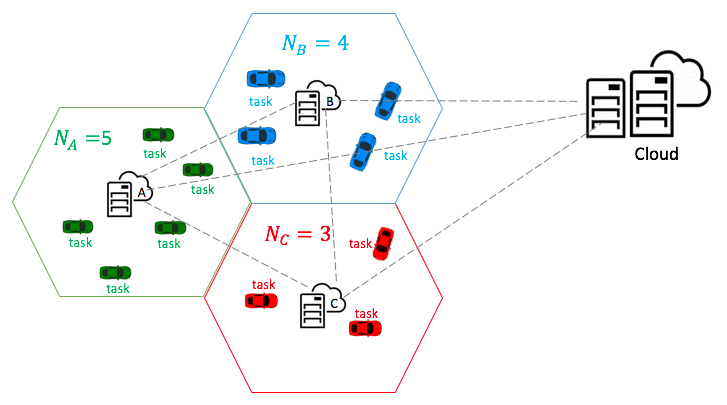
\includegraphics[width=1\linewidth]{images/opt_rep}
\caption{Task Model Example}
\label{opt_rep}
\end{figure}

\begin{figure}[ht!]
\centering
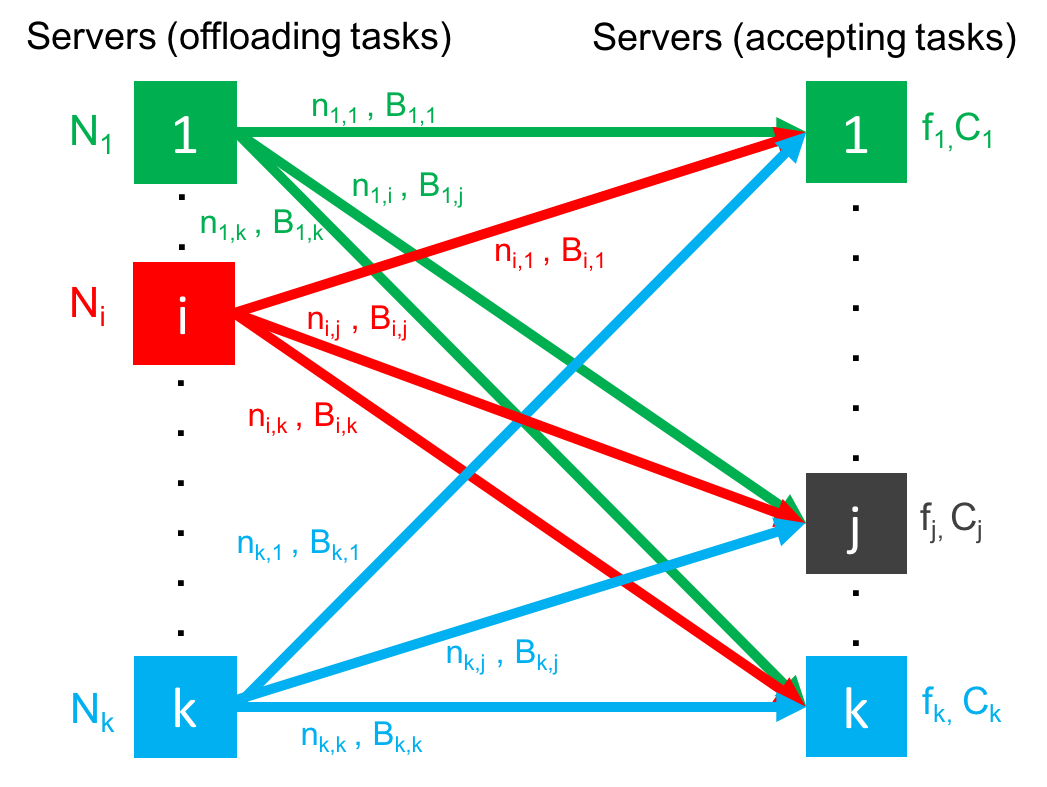
\includegraphics[width=0.8\linewidth]{images/opt_gen}
\caption{Task Model in Fog Computing}
\label{opt_gen}
\end{figure}



\begin{table}[h]
\caption{Parameters \& Variables in the Task Model}
\small
\centering
\begin{tabular}{| m{1cm} |  m{15em} |}
    \hline
    \multicolumn{2}{|l|}{\textbf{Parameters for Servers and Tasks}}\\
    \hline
    $k$ & Number of servers \\
    \hline
    $N_{i}$ & Number of initial tasks for server $i$\\
    \hline
    $B_{ij}$ & Link rate between server $i$ and server $j$ (tasks/sec)\\
    \hline
    $C_{j}$ & Capacity of server $j$ (tasks)\\
    \hline
    $x$ & Number of CPU cycles required for each task (Mcycles)\\
    \hline
    $f_{j}$ & CPU frequency of server $j$ (MHz)\\
    \hline
    $D$ & Deadline for all tasks (sec)\\
    \hline
    $\tau$ & Allowed processing time for each server (sec)\\
    \hline\hline
    \multicolumn{2}{|l|}{\textbf{Optimizing Variables}}\\
    \hline
    $n_{ij}$ & Number of tasks distributed from server $i$ to server $j$\\
    \hline
\end{tabular}
\label{fogsysvar}
\end{table}


 Since we do not know how a server schedules the tasks coming from other servers and the arrival order of those incoming tasks, it is impossible to calculate the completion time for each task that is offloaded to a server. So instead of trying to perform load balancing at the task level, we propose to execute load balancing at the server level by treating the tasks offloaded by other servers as one large aggregated task as illustrated in Figure \ref{opt_agg}. By doing so, we are able to calculate the completion time of the large aggregated task at each server disregarding how that server schedule its tasks and the arrival order of the incoming tasks. 
 


\begin{figure}[ht!]
\centering
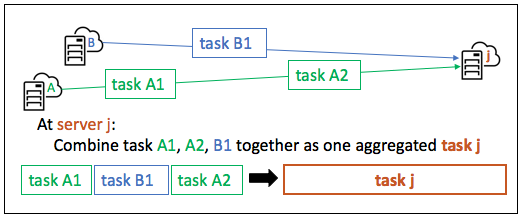
\includegraphics[width=1\linewidth]{images/opt_agg}
\caption{Aggregated Task Example}
\label{opt_agg}
\end{figure}

Now we have defined the concept of an aggregated task at server $j$, we can establish the definitions for the following terms in order to understand the formulation presented next. 
\begin{itemize}[]
\item \textbf{Transmission time for aggregated task at server $j$:} The time for server $i$ to transmit its tasks($n_{ij}$) to server $j$ is $n_{ij}$ divided by the link rate ($B_{ij}$). So the time it takes for all the tasks(aggregated tasks) assigned to server $j$ is the sum of all servers' transmitting time, as shown in (\ref{trans}).
\begin{equation}
\small
\label{trans}
Transmission \ time \ at \ server \ j: \sum\limits_{i=1}^{k} \frac{n_{ij}}{B_{ij}}
\end{equation}


\item \textbf{Turnaround time for aggregated task at server $j$:} The time it takes for server $j$ to process all the tasks offloaded from other servers is calculated by taking the total CPU cycles required, $\sum\limits_{i=1}^{k} n_{ij}*x$, divided by $f_{j}$, the CPU frequency of server $j$, as shown in (\ref{turn}).
\begin{equation}
\small
\label{turn}
Turnaround \ time \ at \ server \ j\ : \sum\limits_{i=1}^{k} \frac{n_{ij}*x}{f_{j}}
\end{equation}

\item
\textbf{Completion time for aggregated task at server $j$:} Completion time at server $j$ is the time it takes to complete its aggregated task. It is the sum of transmission time (\ref{trans}) and turnaroud time (\ref{turn}), as shown in (\ref{comp}).
\begin{equation}
\small
\label{comp}
Completetion \ time \ at \ server \ j\ : \sum\limits_{i=1}^{k} (\frac{n_{ij}}{B_{ij}}+\frac{n_{ij}*x}{f_{j}})
\end{equation}

\item
\textbf{Lateness for aggregated task at server $j$:} Lateness is defined by subtracting completion time (\ref{comp}) with $D$, the deadline, as shown in (\ref{late}).
\begin{equation}
\small
\label{late}
Lateness \ at \ server \ j\ : \left (\sum\limits_{i=1}^{k} (\frac{n_{ij}}{B_{ij}}+\frac{n_{ij}*x}{f_{j}}) \right) - D
\end{equation}

\end{itemize}







\subsection{Problem Formulation}










The objective of the load balancing problem is to minimize deadline misses and total runtime. With the task model in place, we develop a mixed integer program for solving optimal load balancing of tasks across servers. The objective function is shown in (\ref{opt_min}). The optimization goal is to minimize deadline misses and total runtime. To analyze this objective function, first we recognize that $\left (\sum\limits_{i=1}^{k} \frac{n_{ij}}{B_{ij}}+\frac{n_{ij}*x}{f_{j}}\right )-D$ is the lateness of completing aggregated tasks at server $j$, so minimizing this term reflects in minimizing total runtime. Secondly, $v*max\left ( 0, \sum\limits_{i=1}^{k} \frac{n_{ij}}{B_{ij}}+\frac{n_{ij}*x}{f_{j}}\right )$ in (\ref{opt_min}) penalizes tardiness(missed deadlines) of aggregated task at server $j$, so minimizing this term reflects in minimizing deadline misses. Lastly $v$ is used as weighing factor so one can decide to put more emphasis in minimizing deadline misses or total runtime. A more graphical analysis on the objective function (\ref{opt_min}) is shown in Figure \ref{opt_ill}.



\setlength{\arraycolsep}{0.0em}
\small
\begin{eqnarray}
\label{opt_min}
&Min&: \quad \sum_{j=1}^{k}\left [\left (\sum\limits_{i=1}^{k} \frac{n_{ij}}{B_{ij}}+\frac{n_{ij}*x}{f_{j}} \right ) \ - \ D \ + \right.\nonumber\\
&\phantom{min}&\qquad \left.v * max\left ( 0, \sum\limits_{i=1}^{k} \frac{n_{ij}}{B_{ij}}+\frac{n_{ij}*x}{f_{j}}\right )\right ]\\
\label{opt_concpu}
&s.t.& \quad\sum_{i=1}^{k} n_{ij}*x\leq f_{j}*\tau  \qquad for \ j\in \left \{ 1,2,..,k \right \}\\
\label{opt_conc}
&\phantom{s.t.}& \quad\sum_{i=1}^{k} n_{ij}\leq C_{j} \ \ \qquad\quad\quad for \ j\in \left \{ 1,2,..,k \right \}\\
\label{opt_n}
&\phantom{s.t.}& \quad\sum_{j=1}^{k} n_{ij}=N_{i} \  \ \qquad \quad \quad for \ i\in \left \{ 1,2,..,k \right \} \\
\label{opt_int}
&\phantom{s.t.}& \quad n_{ij}\in Z^{+} \qquad \qquad \qquad  for \ i\in \left \{ 1,2,..,k \right \} ,\nonumber\\
&\phantom{s.t.}& \quad\phantom{n_{ij}\in Z^{+}}  \qquad \qquad \qquad for \ j\in \left \{ 1,2,..,k \right \}
\end{eqnarray}
\setlength{\arraycolsep}{5pt}

\begin{figure}[ht!]
\centering
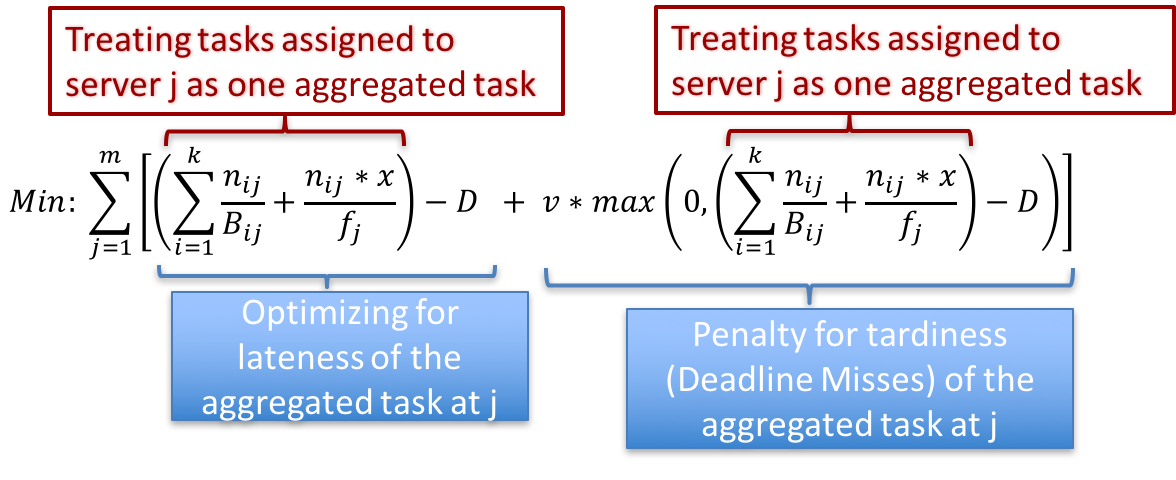
\includegraphics[width=1\linewidth]{images/opt_ill}
\caption{Analysis of Objective Function}
\label{opt_ill}
\end{figure}
\normalsize

The constraints for the optimization are shown from (\ref{opt_concpu}) to (\ref{opt_int}). Constraint (\ref{opt_concpu}) requires that every server has enough CPU cycles available for the tasks offloaded from other servers. Constraint (\ref{opt_conc}) requires the total number of tasks allocated to a server does not exceed its capacity. Constraint (\ref{opt_n}) makes sure that all tasks will be distributed and processed. Constraint (\ref{opt_int}) makes sure a task will not be divided into smaller sub-tasks. Finally we reformulate the objective function (\ref{opt_min}) by introducing $y_{j}$ as shown from (\ref{opt_fstart}) to (\ref{opt_end}) in order to solve the optimization using lp\_solve\cite{lpsolve}.



\setlength{\arraycolsep}{0.0em}
\begin{eqnarray}
\small
\label{opt_fstart}
&Min&: \sum_{j=1}^{k}\left [\left (\sum\limits_{i=1}^{k} \frac{n_{ij}}{B_{ij}}+\frac{n_{ij}*x}{f_{j}} \right ) \ - \ D \ + v * y_{j} \right ]\\
\label{opt_concpu2}
&s.t.& \sum_{i=1}^{k} n_{ij}*x\leq f_{j}*\tau  \qquad for \ j\in \left \{ 1,2,..,k \right \}\\
\label{opt_conc2}
&\phantom{s.t.}& \sum_{i=1}^{k} n_{ij}\leq C_{j} \ \ \qquad\quad\quad for \ j\in \left \{ 1,2,..,k \right \}\\
\label{opt_n2}
&\phantom{s.t.}& \sum_{j=1}^{k} n_{ij}=N_{i} \  \ \qquad \quad \quad for \ i\in \left \{ 1,2,..,k \right \} \\
\label{opt_int2}
&\phantom{s.t.}&  n_{ij}\in Z^{+} \qquad \qquad \qquad  for \ i\in \left \{ 1,2,..,k \right \} ,\nonumber\\
&\phantom{s.t.}& \phantom{n_{ij}\in Z^{+}}  \qquad \qquad \qquad for \ j\in \left \{ 1,2,..,k \right \}\\
\label{opt_y}
&\phantom{s.t.}& y_{j}\geq 0 \ \ \ \qquad\qquad\qquad for \ j\in \left \{ 1,2,..,k \right \}\\
\label{opt_end}
&\phantom{s.t.}& y_{j}\geq \left (\sum\limits_{i=1}^{k} \frac{n_{ij}}{B_{ij}}+\frac{n_{ij}*x}{f_{j}} \right )-D \nonumber\\ 
&\phantom{s.t.}&\qquad\qquad\qquad\qquad\qquad for \ j\in \left \{ 1,2,..,k \right \}
\end{eqnarray}
\setlength{\arraycolsep}{5pt}
\normalsize



\section{Results and Discussion}
\label{s4}

\subsection{Experiment Setup}

Our simulation adopts the system with seven local fog servers as illustrated in Figure \ref{car7} and an additional cloud server. For fog servers, the link rate between server $i$ and server $j$, $B_{ij}$, is randomly drawn from between 16 and 64 tasks per second for $i\ne j$, or $\infty$ for $i=j$, the CPU frequency for server $j$, ${f_{j}}$, is randomly drawn from between 2700 MHz and 3600 MHz, and the capacity of server $j$, $C_{j}$,  is randomly drawn from between 10 and 35 tasks. For the remote cloud server, its initial tasks, $N_{cloud}$ is 0, $B_{icloud}$ is 4 tasks per second, ${f_{cloud}}$ is 4500MHz, and $C_{cloud}$ is $\infty$. For all servers, CPU cycles required per task, $x$, is set at 35 Mcycles, deadline for each task, $D$, is set at 0.5 second, and allowed processing time for each server, $\tau$, is 0.48 second. The system's parameters can be summarized in Table \ref{simvar}.

A taskset is generated by randomly selecting a number for $N_{i}$ from a range of integers which is shown in the first row in Table \ref{ntypes}. By varying the range of integers for $N_{i}$, we can create different loadings for the system. In each experiment, for the same type of loading, taskset generation is performed 100 times, and load balancing optimization is executed for each newly generated taskset. We record all the $N_{i}$ values and so each experiment can be run with the same tasksets. All the experiments were run in the machine with dual quadcore AMD Opteron 2.3 GHz with 16GB memory. The time it takes to execute linear prediction and to solve the optimization on that machine are both less than 0.01 second for all the experiments we run. So the overhead for mobility prediction and load balancing is less than 0.02 second, which is within the overhead budget, calculated by substracting deadline by allowed processing time, $D-\tau=0.5-0.48=0.02$.


\begin{table}[ht!]
\caption{Simulation Parameters}
\centering
\small
\begin{tabular}{| m{0.8cm} | m{1.6cm} | m{15em} |}
    \hline
    \multicolumn{3}{|l|}{\textbf{Simulation Parameters for the System}}\\
    \hline
    $k$ & 8 & Number of servers \\
    \hline
    $x$ & 35 & Number of CPU cycles required for each task (Mcycles)\\
    \hline
    $D$ & 0.5 & Deadline for all tasks (sec)\\
    \hline
    $\tau$ & 0.48 & Allowed processing time for each server (sec)\\
    \hline
    \multicolumn{3}{|l|}{\textbf{Simulation Parameters for Local Fog Servers}}\\
    \hline
    $N_{i}$ & see Table \ref{ntypes} & Number of initial tasks for server $i$\\
    \hline
    \multirow{2}{*}{$B_{ij}$} & [16,64] & Link rate between server $i$ and server $j$ for $i\ne j$ (tasks/sec) \\ \cline{2-3}
    & $\infty$ & Link rate between server $i$ and server $j$ for $i=j$ (tasks/sec) \\
    % $B_{ij}$ & [16,64] & Link rate between server $i$ and server $j$ (tasks/sec)\\
    \hline
    $C_{j}$ & [10,35] & Capacity of server $j$ (tasks)\\
    \hline
    $f_{j}$ & [2700,3600] & CPU frequency of server $j$ (MHz)\\
    \hline
    \multicolumn{3}{|l|}{\textbf{Simulation Parameters for Cloud Server}}\\
    \hline
    $N_{cloud}$ & 0 & Number of inital tasks for cloud server\\
    \hline
    $B_{icloud}$ & 4 & Link rate between server $i$ and cloud server (tasks/sec)\\
    \hline
    $C_{cloud}$ & $\infty$ & Capacity of cloud server (tasks)\\
    \hline
    $f_{cloud}$ & 4500 & CPU frequency of cloud server (MHz)\\
    \hline\hline
    \multicolumn{2}{|l|}{\textbf{Optimizing Variables}}\\
    \hline
    $n_{ij}$ & solved with optimization & Number of tasks distributed from server $i$ to server $j$\\
    \hline
\end{tabular}
\label{simvar}
\end{table}

\begin{table}[h]
\caption{Types of Workloads}
\small
\centering
\begin{tabular}{|m{1cm}|m{1cm}|m{1cm}|m{1cm}|m{1cm}|m{1cm}|}
    \hline
    Range for $N_{i}$ (tasks)& [10,26] & [10,28] & [10,30] & [10,32] & [10,34] \\ \hline
    Total number of tasks & 12687 & 13472 & 14143 & 14739 & 15051 \\ \hline
\end{tabular}
\label{ntypes}
\end{table}

\subsection{Deadline Misses vs Total Runtime}

In this experiment, we focus on the varying $v$, the weighing parameter in the optimization formulation presented. According to our objective function (\ref{opt_fstart}), a greater $v$ value should result in fewer deadline misses with higher total runtime. We verify such trend by running experiment with different $v$ and gather the results for deadline misses and total runtime respectively, as shown in Figure \ref{res_opt_vs_opt_md} and Figure \ref{res_opt_vs_opt_time}. From the figures, we observe that a larger $v$ does result in fewer deadline misses and higher total runtime.


\begin{figure}[h!]
\centering
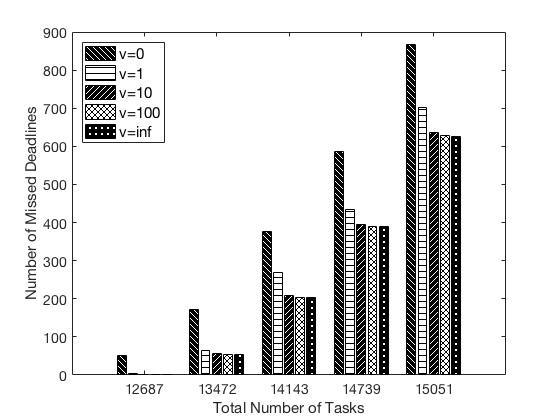
\includegraphics[width=1\linewidth]{images/res_opt_vs_opt_mdp}
\caption{Deadline Misses Comparison with Different $v$ }
\label{res_opt_vs_opt_md}
\end{figure}


\begin{figure}[h!]
\centering
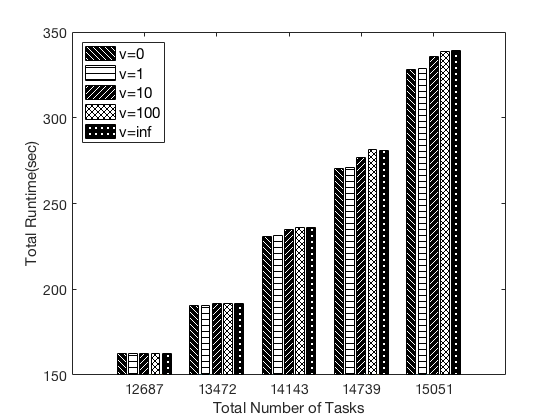
\includegraphics[width=1\linewidth]{images/res_opt_vs_opt_timep}
\caption{Total Runtime Comparison with Different $v$ }
\label{res_opt_vs_opt_time}
\end{figure}


\subsection{Comparison with Other Load Balancing Algorithms}



We compare our optimization result with local static, a simple load balancing method, and three other commonly used load balancing algorithms: weighted round robin, active monitoring and throttled load balancer\cite{wrr}\cite{amt}\cite{amt2}. In local static load balancing, each server with initial tasks exceed its capacity will transfer all the overloading tasks to the cloud server. Weighted round robin is implemented by assigning high weights for local servers that have not reached their maximum capacity. The cloud server will have a higher weight than a local server only when that server reaches its maximum capacity. Active monitoring load balancing is implemented by having each task assigned to the local server that has the highest remaining capacity, the algorithm will only assign to the cloud server when all the local servers are full. In the throttled load balancer, each task is assigned based on the most suitable server available, so the server with lowest completion time and has not reached its maximum capacity will be assigned with the new task. Again, a cloud server will be utilized only when none of the local servers are available. The comparisons are shown in Figure \ref{res_opt_vs_lb_ls_md} and Figure \ref{res_opt_vs_lb_ls_time}. Local static does not utilize any available local server so it is not surprising that local static is outperformed by more than 50\% in every case. On the other hand, our optimization has the least deadline misses and total runtime for every case. The numerical results for deadline misses is presented in Table \ref{good}. From Table \ref{good}, at a lighter load of 13472 tasks, our optimization outperforms throttled load balancer which has the second least deadline misses, by almost 50\%, but as the load of the system increases, the improvement brought by optimization starts to decrease. At the heaviest load of 15051 tasks, the improvment our optimization can bring drops to about 25\%. The reason being a heavy loaded system has fewer available options for task distributing, thus the potential for a better performance gets smaller as more load is added to the system.




 
% \begin{figure}[ht!]
% \centering
% 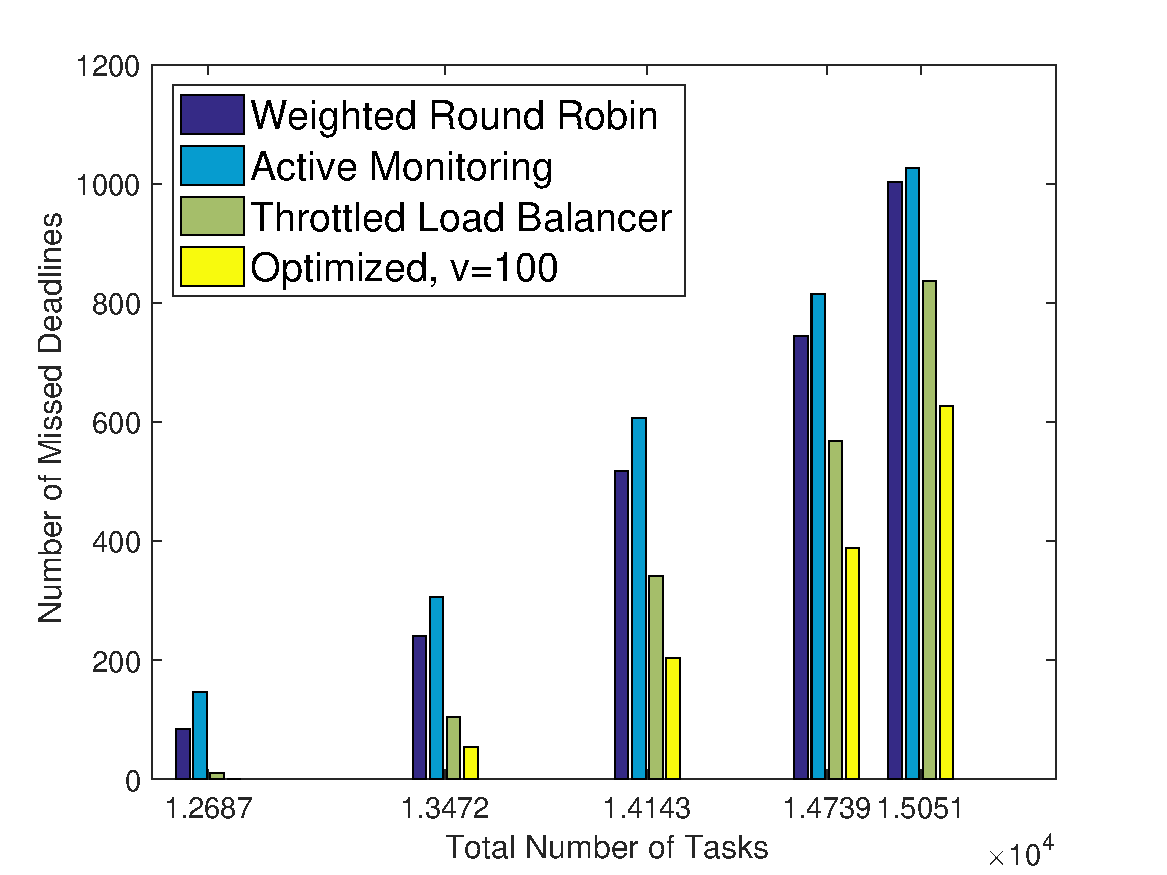
\includegraphics[width=1\linewidth]{images/res_opt_vs_lb_md}
% \caption{Deadline Misses Comparison with Other Load Balancing Algorithms}
% \label{res_opt_vs_lb_md}
% \end{figure}


% \begin{figure}[ht!]
% \centering
% 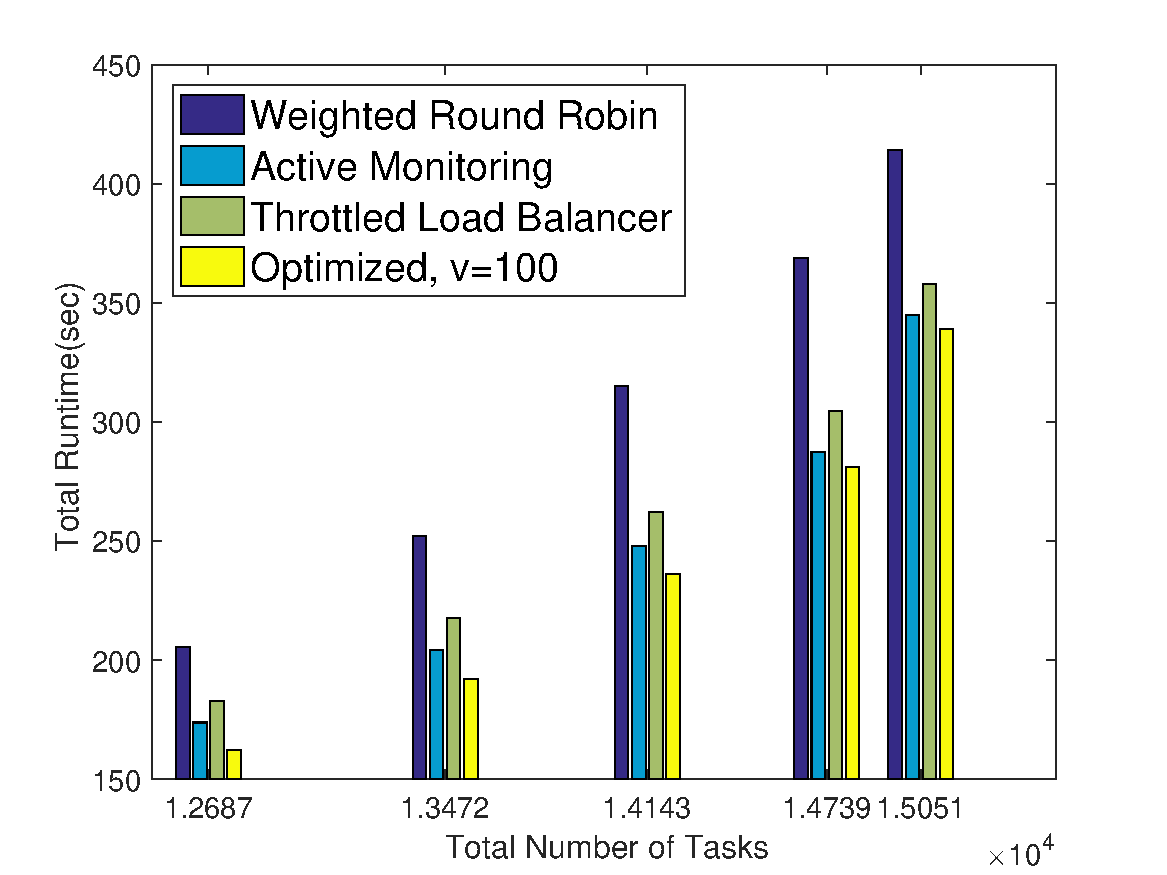
\includegraphics[width=1\linewidth]{images/res_opt_vs_lb_time}
% \caption{Total Runtime Comparison with Other Load Balancing Algorithms}
% \label{res_opt_vs_lb_time}
% \end{figure}

 
\begin{figure}[ht!]
\centering
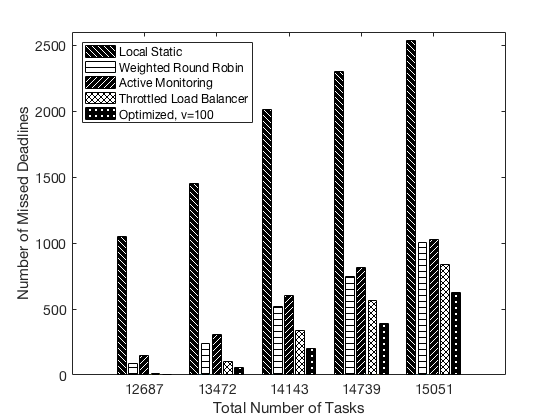
\includegraphics[width=1\linewidth]{images/res_opt_vs_lb_ls_mdp}
\caption{Deadline Misses Comparison with Other Load Balancing Algorithms}
\label{res_opt_vs_lb_ls_md}
\end{figure}


\begin{figure}[ht!]
\centering
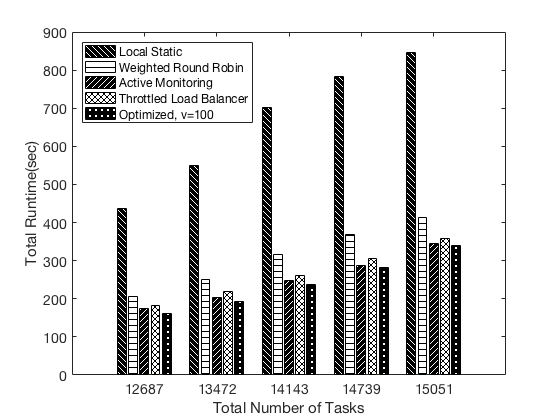
\includegraphics[width=1\linewidth]{images/res_opt_vs_lb_ls_timep}
\caption{Total Runtime Comparison with Other Load Balancing Algorithms}
\label{res_opt_vs_lb_ls_time}
\end{figure}

\begin{table}[h]
\small
\caption{Missed Deadlines Counts}
\centering
\begin{tabular}{|m{1.5cm}|m{0.75cm}|m{0.75cm}|m{0.75cm}|m{0.75cm}|m{0.75cm}|}
    \hline
    \textbf{Total number of tasks} & \textbf{12687} & \textbf{13472} & \textbf{14143} & \textbf{14739} & \textbf{15051} \\ 
    \hline
    Optimized, $v$=100 & 0 & 54 & 204 & 389 & 627 \\
    \hline
    Local Static & 1052 & 1454 & 2011 & 2300 & 2535 \\
    \hline
    Weighted Round Robin & 85 & 240 & 517 & 745& 1003 \\
    \hline
    Active Monitoring & 147 & 306 & 606 & 815& 1026 \\
    \hline
    Throttled Load Balancer & 11 & 104 & 341 & 568& 837 \\
    \hline
\end{tabular}
\label{good}
\end{table}

% \begin{table}[h]
% \small
% \caption{Missed Deadlines Counts}
% \centering
% \begin{tabular}{|m{1.5cm}|m{0.75cm}|m{0.75cm}|m{0.75cm}|m{0.75cm}|m{0.75cm}|}
%     \hline
%     \textbf{Total number of tasks} & \textbf{12687} & \textbf{13472} & \textbf{14143} & \textbf{14739} & \textbf{15051} \\ 
%     \hline
%     Optimized, $v$=100 & 0 & 54 & 204 & 389 & 627 \\
%     \hline
%     Local Static & 1052 & 1454 & 2011 & 2300 & 2535 \\
%     \hline
%     Weighted Round Robin & 85 & 240 & 517 & 745& 1003 \\
%     \hline
%     Active Monitoring & 147 & 306 & 606 & 815& 1026 \\
%     \hline
%     Throttled Load Balancer & 11 & 104 & 341 & 568& 837 \\
%     \hline
% \end{tabular}
% \label{good}
% \end{table}


% \begin{table}[h]
% \small
% \caption{Deadline Misses ratio - deadline misses/total tasks, $v$=100}
% \centering
% \begin{tabular}{|m{1.5cm}|m{0.75cm}|m{0.75cm}|m{0.75cm}|m{0.75cm}|m{0.75cm}|}
%     \hline
%     \textbf{Total number of tasks} & \textbf{12687} & \textbf{13472} & \textbf{14143} & \textbf{14739} & \textbf{15051} \\  
%     \hline
%     Optimized, $v$=100 & 0\% & .40\% & 1.44\% & 2.64\% & 4.17\% \\
%     \hline
%     Local Static & 8.29\% & 10.79\% & 14.2\% & 15.6\% & 16.8\% \\
%     \hline
%     Weighted Roung Robin & 0.67\% & 1.78\% & 3.66\% & 5.05\% & 6.66\% \\
%     \hline
%     Active Monitoring  & 1.16\% & 2.27\% & 4.28\% & 5.53\% & 6.82\% \\    
%     \hline
%     Thorttled Load Balancer & 0.087\% & 0.77\% & 2.41\% & 3.85\% & 5.56\% \\
%     \hline
% \end{tabular}
% \label{bad}
% \end{table}



% \begin{table}[h]
% \small
% \caption{Deadline Misses Comparison to Optimized \%, $v$=100}
% \centering
% \begin{tabular}{|m{1.5cm}|m{0.75cm}|m{0.75cm}|m{0.75cm}|m{0.75cm}|m{0.75cm}|}
%     \hline
%     \textbf{Total number of tasks} & \textbf{12687} & \textbf{13472} & \textbf{14143} & \textbf{14739} & \textbf{15051} \\ 
%     \hline
%     Local Static & 100\% & 96.3\% & 89.9\% & 83.1\% & 75.3\% \\
%     \hline
%     Weighted Roung Robin  & 100\% & 77.5\% & 60.5\% & 48.8\%& 37.5\% \\
%     \hline
%     Active Monitoring  & 100\% & 82.4\% & 66.3\% & 52.3\%& 38.9\% \\
%     \hline
%     Thorttled Load Balancer & 100\% & 48.1\% & 40.2\% & 31.5\%& 25.1\% \\
%     \hline
% \end{tabular}
% \label{best}
% \end{table}

















%\section{Results}
% \section{Discussion}
Expect about 2 pages.

% JP to lead.

This is the discussion that follows the results.  It's possible that I may
combine these two sections into a single session (results and discussion). This
is where we point out the differences in results - where individual hypervisors
started to trip up, what characteristics they exhibited, etc.


\section{Conclusion and Future Work}
\label{s5}



In this work, we propose a task scheduling model for connected car system in fog computing that brings task scheduling from device level to server level, which reduces the amount of computations required to perform load balancing. We also formulate a load balancing optimization problem that minimizes deadline misses and total runtime. We show that our optimization outperforms some common load balancing algorithms such as weighted round robin, active monitoring, and throttled load balancer. There are many potentials and ideas to expand on this topic including take energy consumption into consideration, vary the parameters dynamically, or implement applications with real workloads. We look forward to pursuing more research in this topic as the development of fog computing and connected car systems continues.


% Adjust this to balance last page if not using package
\IEEEtriggeratref{24}
\bibliography{socc2018}
\bibliographystyle{./IEEEtranBST/IEEEtran}

\end{document}

